%& C:\Users\lizil\AppData\Roaming\TikzEdt\TikzEdt\023~1.0\TEMP_H~1
\begin{document}
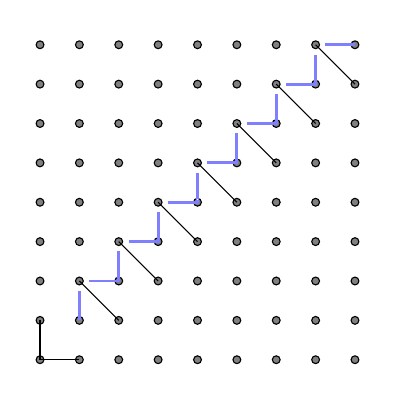
\begin{tikzpicture}
\tikzstyle{dot}=[draw,circle,fill=gray,scale=0.3];
\foreach \x in {0,...,8}
	\foreach \y in {0,...,8}
		\node[dot] at (\x*0.5,\y*0.5) {};

\draw (0,0) -- (0,0.5);
\draw (0,0) -- (0.5,0);
\draw (0.5,1) node (v1) {} -- (1,0.5);
\draw (1,1.5) node (v2) {} -- (1.5,1);
\draw (1.5,2) node (v3) {} -- (2,1.5);
\draw (2,2.5) node (v4) {} -- (2.5,2);
\draw (2.5,3) node (v5) {} -- (3,2.5);
\draw (3,3.5) node (v6) {} -- (3.5,3);
\draw (3.5,4) node (v8) {} -- (4,3.5);

\draw[draw=blue!50,line width=1pt] (0.5,0.5) -- (v1) -- (1,1) -- (v2) -- (1.5,1.5) -- (v3) -- (2,2) -- (v4) -- (2.5,2.5) -- (v5) -- (3,3) -- (v6) -- (3.5,3.5) node (v7) {}-- (v8) -- (4,4);

\usetikzlibrary{calc}
\pgftransformreset
\node[inner sep=0pt,outer sep=0pt,minimum size=0pt,line width=0pt,text width=0pt,text height=0pt] at (current bounding box) {};
%add border to avoid cropping by pdflibnet
\foreach \border in {0.1}
  \useasboundingbox (current bounding box.south west)+(-\border,-\border) rectangle (current bounding box.north east)+(\border,\border);
\newwrite\metadatafile
\immediate\openout\metadatafile=\jobname_BB.txt
\path
  let
    \p1=(current bounding box.south west),
    \p2=(current bounding box.north east)
  in
  node[inner sep=0pt,outer sep=0pt,minimum size=0pt,line width=0pt,text width=0pt,text height=0pt,draw=white] at (current bounding box) {
\immediate\write\metadatafile{\p1,\p2}
};
\immediate\closeout\metadatafile
\end{tikzpicture}

\end{document}
